
\sujet{Stochastic watershed}
\index{Mathematical Morphology:Watershed}

\section{Stochastic Watershed}
The algorithm of the stochastic watershed to segment an image $I$ can be summarized by the following steps:
\begin{enumerate}
 \item Generate $n$ random points from a Poisson point process.
 \item Use these points as markers and perform a constrained watershed on the image $I$.
 \item Repeat $m$ times these first two steps.
 \item Evaluate the probability density function (the use of \minline{ksdensity} can be considered) of these $m$ realizations.
 \item Segment the obtained pdf via a classical watershed.
\end{enumerate}

\begin{qbox}
 Code a \matlabregistered{} function that takes 3 arguments: $n$, $m$ and $I$, and returns the segmented image.
\end{qbox}

\section{Open question}
A serie of corneal images is given in addition to a manual segmentation (Fig. \ref{fig:endothelium}). 
\begin{figure}[htbp]
 \centering
 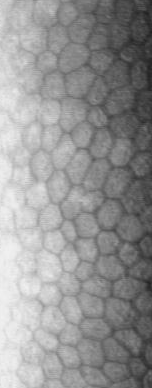
\includegraphics[width=4cm]{10.png}
 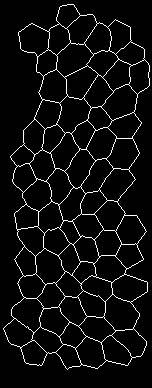
\includegraphics[width=4cm]{expert_10.png}
 \caption{Human corneal endothelium in specular microscopy and manual segmentation of the cells.}
 \label{fig:endothelium}
\end{figure}


\begin{qbox}
 \begin{itemize}
  \item Apply the previous segmentation algorithm on these images.
 \end{itemize}
\end{qbox}

The drawback of this segmentation algorithm is the choice of $n$. 
\begin{qbox}
Propose a method in order to evaluate the best $n$ and $m$. The optimal segmentation is available from the campus website.
\end{qbox}

